\sweExpl{[Vad gjorde du? Hur gick det till? – Välj lämplig rubrik (“Genomförande”, “Konstruktion”, ”Utveckling”  eller annat]}


\engExpl{What have you done? How did you do it? What design decisions did you make? How did what you did help you to meet your goals?}
\sweExpl{Vad du har gjort? Hur gjorde du det? Vilka designval gjorde du?\\
Hur kom det du hjälpte dig att uppnå dina mål?}

% the following sets the TOC entry to break after the & - note you have to include the first letter of the following word as it get swolled by the \texorpdfstring{}{} processing
\section[Hardware/Software design …/Model/Simulation model \&\texorpdfstring{\\}{ p} parameters/…]{Hardware/Software design …/Model/Simulation model \& parameters/…}
\sweExpl{Hårdvara / Mjukvarudesign ... / modell / Simuleringsmodell och parametrar / …}

Figure~\ref{fig:homepageicon} shows a simple icon for a home page. The time
to access this page when served will be quantified in a series of
experiments. The configurations that have been tested in the test bed are
listed in Table~\ref{tab:configstested}. In \SI{7.0}{\percent} of cases, there was an error indicating xxxxx.

\sweExpl{Figur~\ref{fig:homepageicon}  visar en enkel ikon för en hemsida. Tiden för att få tillgång till den här sidan när den laddas kommer att kvantifieras i en serie experiment. De konfigurationer som har testats i provbänk listas ini tabell~\ref{tab:configstested}.\\
Vad du har gjort? Hur gjorde du det? Vilka designval gjorde du?}
 
\begin{figure}[!ht]
  \begin{center}
    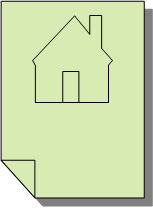
\includegraphics[width=0.25\textwidth]{figures/Homepage-icon.png}
  \end{center}
  \caption{Homepage icon}
  \label{fig:homepageicon}
\end{figure}

\begin{table}[!ht]
  \begin{center}
    \caption{Configurations tested}
    \label{tab:configstested}
    \resizebox{\columnwidth}{!}{%
    \begin{tabular}{l|c} % <-- Alignments: 1st column left, 2nd middle and 3rd right, with vertical lines in between
      \textbf{Configuration} & \textbf{Description} \\
      \hline
      1 & Simple test with one server\\
      2 & Simple test with one server\\
    \end{tabular}
    }
  \end{center}
\end{table}
\sweExpl{Testade konfigurationer}

\section{Implementation …/Modeling/Simulation/…}
\label{sec:implementationDetails}
\sweExpl{Implementering … / modellering / simulering / …}

Two commonly used simulators are:
\begin{description}[labelwidth =\widthof{\textbf{ns-2 or ns-3 simulator}}, leftmargin = !]
    \item[\textbf{Mininet}] This simulator uses traffic control (\texttt{tc}) to simulate network devices connected by links with specific bandwidth, packet loss rates, qdisc methods, etc.
    
    
    \item[\textbf{ns-2 or ns-3 simulator}] These simulators are very useful for simulating wireless communication links between moving devices. You can specify the mobility patterns of the nodes.
\end{description}

\subsection{Some examples of coding}
\engExpl{This section is simply to show some example of how you can include code in your thesis - this is not a section you would have in your thesis.}
\sweExpl{Det här avsnittet är helt enkelt för att visa ett exempel på hur du kan inkludera kod i ditt examensarbete - det här är inte ett avsnitt du skulle ha i ditt examensarbete.}

Listing~\ref{lst:helloWorldInC} shows an example of a simple program written
in C code.

\begin{lstlisting}[language={C}, caption={Hello world in C code}, label=lst:helloWorldInC]
int main() {
printf("hello, world");
return 0;
}
\end{lstlisting}


In contrast, Listing~\ref{lst:programmes} is an example of code in Python to
get a list of all of the programs at KTH.

\lstset{extendedchars=true}  %% This allows characters codes in the range 128-255
\begin{lstlisting}[language={Python}, caption={Using a python program to
    access the KTH API to get all of the programs at KTH}, label=lst:programmes]
KOPPSbaseUrl = 'https://www.kth.se'

def v1_get_programmes():
    global Verbose_Flag
    #
    # Use the KOPPS API to get the data
    # note that this returns XML
    url = "{0}/api/kopps/v1/programme".format(KOPPSbaseUrl)
    if Verbose_Flag:
        print("url: " + url)
    #
    r = requests.get(url)
    if Verbose_Flag:
        print("result of getting v1 programme: {}".format(r.text))
    #
    if r.status_code == requests.codes.ok:
        return r.text           # simply return the XML
    #
    return None
\end{lstlisting}
\FloatBarrier

\subsection{Some examples of figures in tikz}
\engExpl{This section is simply to show some example of how you can draw your own figures for in your thesis - this is not a section you would have in your thesis.}
\sweExpl{Det här avsnittet är helt enkelt för att visa ett exempel på hur du kan rita dina egna figurer i ditt examensarbete – det här är inte ett avsnitt du skulle ha i ditt examensarbete.}

These figures are just some examples to show that you can draw your own figures for in your thesis. This has two advantages: \first you do not have to worry about copyrights -- as these are your own figures and \Second the text is now readable and not simply a picture of text -- so screen readers can read the figure's contents to someone who is listening to the contents of your thesis.

\subsubsection{Azure's Form Recognizer}
\Cref{fig:processAnInvoice} shows the processing of key-value extraction from a PDF document using Azure's Form Recognizer. 

\tikzset{
    processBox/.style={rectangle, rounded corners, minimum width=3cm, minimum height=1cm,text centered, font=\sffamily, draw=black, fill=red!20},
    largeBox/.style={rectangle, rounded corners, minimum width=3cm, minimum height=4cm,text centered, draw=black}
}
\begin{figure}[!ht]
\resizebox{1.1\textwidth}{!}{%
\begin{tikzpicture}
[align=left,node distance=2cm]

\node (document) [tape,tape bend top=none,draw,font=\sffamily] {PDF\\Document};
\node (GDM) [processBox,  right=0.5cm of document] {OCR};
\node (OCRoutput) [largeBox, right=1cm of GDM] {OCR output};

\node (kvp) [tape,tape bend top=none,draw,font=\sffamily, below=0.25cm of OCRoutput.north] {key-value\\pairs};
\node (entities) [tape,tape bend top=none,draw,font=\sffamily, above=0.35cm of OCRoutput.south] {Entities};
\node (Manual) [processBox, right=1cm of kvp] {Analyze the extracted\\key-value pairs};
\draw [-latex](document) --  (GDM);
\draw [-latex](kvp) --  (Manual);
\path[ draw
     , -latex'] let \p1=(GDM.east), \p2=(kvp.west) in (GDM.east) -- +(0.25*\x2-0.25*\x1, \y1) -- +(0.5*\x2-0.5*\x1, \y2) -- (kvp.west);
\path[ draw
     , -latex'] let \p1=(GDM.east), \p2=(kvp.west), \p3=(entities.west) in (GDM.east) --  +(0.25*\x2-0.25*\x1, \y1) -- +(0.5*\x3-0.5*\x1, \y3) -- (entities.west);
\end{tikzpicture}
}
\caption{The processing of key-value extraction from a PDF document using Azure's Form Recognizer}
  \label{fig:processAnInvoice}
\end{figure}
\FloatBarrier
\subsubsection{Hyper-V with Containers}
 \Cref{fig:hyperVcontainers} shows how Hyper-V deals with containers.
 
 \tikzset{
    container/.style={rectangle, rounded corners, minimum width=2cm, minimum height=1cm,text centered, draw=black, fill=blue!20},
    containerization/.style={rectangle, rounded corners, minimum width=13.25cm, minimum height=1cm,text centered, draw=black, fill=blue!20},
    hypervisor/.style={rectangle, rounded corners, minimum width=13.25cm, minimum height=1cm,text centered, draw=black, fill=red!20},
    os/.style={rectangle, rounded corners, minimum width=13.25cm, minimum height=1cm,text centered, draw=black, fill=orange!20},
    guestos/.style={rectangle, rounded corners, minimum width=2cm, minimum height=1cm,text centered, draw=black, fill=orange!40},
    infrastructure/.style={rectangle, rounded corners, minimum width=13.25cm, minimum height=1cm,text centered, draw=black, fill=green!20},
    hos/.style={rectangle, rounded corners, minimum width=6cm, minimum height=1cm,text centered, draw=black, fill=orange!20},
    kernel/.style={rectangle, rounded corners, minimum width=6cm, minimum height=1cm,text centered, draw=black, fill=purple!20},
    services/.style={rectangle, rounded corners, minimum width=3cm, minimum height=1cm,text centered, draw=black, fill=pink!20]}
}

\begin{figure}[ht!]
    \centering
\resizebox{1\textwidth}{!}{%
\begin{tikzpicture}
[align=center,node distance=2cm]

\node (Infrastructure) [infrastructure, text width=13cm, text centered] {Infrastructure};
\node (OS1) [hos, anchor=north west, align=left, above=1.5cm of Infrastructure.north west, anchor=north west, text width=6cm, text centered] {Host OS};

\node (OS2) [hos, anchor= west, align=left, right=0.5cm of OS1.east, text width=6cm, anchor= west, text centered] {Host OS};

\node (Kernel1) [kernel, anchor=north west, align=left, above=1.5cm of OS1.north east, anchor=north east, text width=3cm, text centered] {Kernel};

\node (Kernel2) [kernel, anchor=north west, align=left, above=1.5cm of OS2.north east, anchor=north east, text width=3cm, text centered] {Kernel};

\node (ServiceA) [container, anchor=east, above=1 cm of Kernel1.east, anchor=east] {Services};
\node (AppA) [container,  left=0.25cm of ServiceA] {App 1};

\node (ServiceB) [container, anchor=east, above=1 cm of Kernel2.east, anchor=east] {Services};
\node (AppB) [container,  left=0.25cm of ServiceB] {App 2};
%\node (AppC) [container,  right=0.25cm of AppB] {App 3};

\draw[black,thick,dashed] ($(OS2.north west)+(-0.3,3.75)$)  rectangle ($(OS2.south east)+(0.5,-0.3)$);
\node[text width=5cm, text=red, above=0.1cm of ServiceB] 
    {\textbf{Container}};

\draw[red,thick,dotted] ($(Kernel2.north west)+(-0.3,1.6)$)  rectangle ($(Kernel2.south east)+(0.3,-0.3)$);
\node[text width=5cm, text=black, above=0.8cm of ServiceB] 
    {\textbf{VM}};
\end{tikzpicture}
}
    \caption{Hyper-V with containers}
    \label{fig:hyperVcontainers}
\end{figure}
\FloatBarrier
\subsubsection{\glsfmtshort{VM} versus Containers}
\Cref{fg:vmsVersusContainers} shows a comparison of virtual machines (VMs) versus containers.

\begin{figure*}[ht!]
    \centering
    \begin{subfigure}[t]{0.5\textwidth}
        \centering
\resizebox{1\textwidth}{!}{%
\begin{tikzpicture}
[align=left,node distance=2cm]

\node (AppA) [container,align=left] {App 1};
\node (AppB) [container,  right=0.25cm of AppA] {App 2};
\node (AppC) [container,  right=0.25cm of AppB] {App 3};

\node (GosA) [guestos,align=left,  below=0.25cm of AppA.south west,anchor=north west] {Guest OS};
\node (GosB) [guestos,  right=0.25cm of GosA] {Guest OS};
\node (GosC) [guestos,  right=0.25cm of GosB] {Guest OS};

\draw [decoration={brace,amplitude=0.5em},decorate, ultra thick,gray, transform canvas={xshift = 0.5cm}]
       (AppC.north -| AppC.east) -- (GosC.south -| AppC.east);
\node[text width=5cm,  right=1cm of GosC.north east] 
    {\textbf{VMs}};

\node (Hypervisor) [hypervisor, anchor=north west, align=left, below=0.25cm of GosA.south west, anchor=north west, text width=13cm, text centered] {Hypervisor};

\node (OS) [os, anchor=north west, align=left, below=0.25cm of Hypervisor.south west, anchor=north west, text width=13cm, text centered] {Host OS};

\node (Infrastructure) [infrastructure, anchor=north west, align=left, below=0.25cm of OS.south west, anchor=north west, text width=13cm, text centered] {Infrastructure};


\end{tikzpicture}
}
        \caption{VM}
    \end{subfigure}%
    ~ 
    \begin{subfigure}[t]{0.5\textwidth}
        \centering
        \resizebox{1\textwidth}{!}{%
\begin{tikzpicture}
[align=left,node distance=2cm]

\node (AppA) [container,align=left] {App 1};
\node (AppB) [container,  right=0.25cm of AppA] {App 2};
\node (AppC) [container,  right=0.25cm of AppB] {App 3};
\node[text width=5cm,  right=0.25cm of AppC] 
    {\textbf{Apps running in Containers}};


\node (Containerization) [containerization, anchor=north west, align=left, below=0.25cm of AppA.south west, anchor=north west, text width=13cm, text centered] {Docker Engine};

\node (OS) [os, anchor=north west, align=left, below=0.25cm of Containerization.south west, anchor=north west, text width=13cm, text centered] {Host OS};

\node (Infrastructure) [infrastructure, anchor=north west, align=left, below=0.25cm of OS.south west, anchor=north west, text width=13cm, text centered] {Infrastructure};


\end{tikzpicture}
}
        \caption{Containers}
    \end{subfigure}
    \caption{Virtual machines (VMs) versus Containers}
    \label{fg:vmsVersusContainers}
\end{figure*}
